\documentclass[english, 11 pt, class=article, crop=false]{standalone}
\usepackage[T1]{fontenc}
\usepackage[utf8]{luainputenc}
\usepackage{lmodern} % load a font with all the characters
\usepackage{geometry}
\geometry{verbose,paperwidth=16.1 cm, paperheight=24 cm, inner=2.3cm, outer=1.8 cm, bmargin=2cm, tmargin=1.8cm}
\setlength{\parindent}{0bp}
\usepackage{import}
\usepackage[subpreambles=false]{standalone}
\usepackage{amsmath}
\usepackage{amssymb}
\usepackage{esint}
\usepackage{babel}
\usepackage{tabu}
\makeatother
\makeatletter

\usepackage{titlesec}
\usepackage{ragged2e}
\RaggedRight
\raggedbottom
\frenchspacing

% Norwegian names of figures, chapters, parts and content
\addto\captionsenglish{\renewcommand{\figurename}{Figur}}
\makeatletter
\addto\captionsenglish{\renewcommand{\chaptername}{Kapittel}}
\addto\captionsenglish{\renewcommand{\partname}{Del}}

\addto\captionsenglish{\renewcommand{\contentsname}{Innhald}}

\usepackage{graphicx}
\usepackage{float}
\usepackage{subfig}
\usepackage{placeins}
\usepackage{cancel}
\usepackage{framed}
\usepackage{wrapfig}
\usepackage[subfigure]{tocloft}
\usepackage[font=footnotesize]{caption} % Figure caption
\usepackage{bm}
\usepackage[dvipsnames, table]{xcolor}
\definecolor{shadecolor}{rgb}{0.105469, 0.613281, 1}
\colorlet{shadecolor}{Emerald!15} 
\usepackage{icomma}
\makeatother
\usepackage[many]{tcolorbox}
\usepackage{multicol}
\usepackage{stackengine}

% For tabular
\addto\captionsenglish{\renewcommand{\tablename}{Tabell}}
\usepackage{array}
\usepackage{multirow}
\usepackage{longtable} %breakable table

% Ligningsreferanser
\usepackage{mathtools}
\mathtoolsset{showonlyrefs}

% index
\usepackage{imakeidx}
\makeindex[title=Indeks]

%Footnote:
\usepackage[bottom, hang, flushmargin]{footmisc}
\usepackage{perpage} 
\MakePerPage{footnote}
\addtolength{\footnotesep}{2mm}
\renewcommand{\thefootnote}{\arabic{footnote}}
\renewcommand\footnoterule{\rule{\linewidth}{0.4pt}}
\renewcommand{\thempfootnote}{\arabic{mpfootnote}}

%colors
\definecolor{c1}{cmyk}{0,0.5,1,0}
\definecolor{c2}{cmyk}{1,0.25,1,0}
\definecolor{n3}{cmyk}{1,0.,1,0}
\definecolor{neg}{cmyk}{1,0.,0.,0}

% Lister med bokstavar
\usepackage[inline]{enumitem}

\newcounter{rg}
\numberwithin{rg}{chapter}
\newcommand{\reg}[2][]{\begin{tcolorbox}[boxrule=0.3 mm,arc=0mm,colback=blue!3] {\refstepcounter{rg}\phantomsection \large \textbf{\therg \;#1} \vspace{5 pt}}\newline #2  \end{tcolorbox}\vspace{-5pt}}

\newcommand{\regg}[2]{\begin{tcolorbox}[boxrule=0.3 mm,arc=0mm,colback=blue!3] {\large \textbf{#1} \vspace{5 pt}}\newline #2  \end{tcolorbox}\vspace{-5pt}}

\newcommand\alg[1]{\begin{align} #1 \end{align}}

\newcommand\eks[2][]{\begin{tcolorbox}[boxrule=0.3 mm,arc=0mm,enhanced jigsaw,breakable,colback=green!3] {\large \textbf{Eksempel #1} \vspace{5 pt}\\} #2 \end{tcolorbox}\vspace{-5pt} }

\newcommand{\st}[1]{\begin{tcolorbox}[boxrule=0.0 mm,arc=0mm,enhanced jigsaw,breakable,colback=yellow!12]{ #1} \end{tcolorbox}}

\newcommand{\spr}[1]{\begin{tcolorbox}[boxrule=0.3 mm,arc=0mm,enhanced jigsaw,breakable,colback=yellow!7] {\large \textbf{Språkboksen} \vspace{5 pt}\\} #1 \end{tcolorbox}\vspace{-5pt} }

\newcommand{\sym}[1]{\colorbox{blue!15}{#1}}

\newcommand{\info}[2]{\begin{tcolorbox}[boxrule=0.3 mm,arc=0mm,enhanced jigsaw,breakable,colback=cyan!6] {\large \textbf{#1} \vspace{5 pt}\\} #2 \end{tcolorbox}\vspace{-5pt} }

\newcommand\algv[1]{\vspace{-11 pt}\begin{align*} #1 \end{align*}}

\newcommand{\regv}{\vspace{5pt}}
\newcommand{\mer}{\textsl{Merk}: }
\newcommand\vsk{\vspace{11pt}}
\newcommand\vs{\vspace{-11pt}}
\newcommand\vsabc{\vspace{-5pt}}
\newcommand\vsb{\vspace{-16pt}}
\newcommand\sv{\vsk \textbf{Svar:} \vspace{4 pt}\\}
\newcommand\br{\\[5 pt]}
\newcommand{\fpath}[1]{../fig/#1}
\newcommand\algvv[1]{\vs\vs\begin{align*} #1 \end{align*}}
\newcommand{\y}[1]{$ {#1} $}
\newcommand{\os}{\\[5 pt]}
\newcommand{\prbxl}[2]{
	\parbox[l][][l]{#1\linewidth}{#2
}}
\newcommand{\prbxr}[2]{\parbox[r][][l]{#1\linewidth}{
		\setlength{\abovedisplayskip}{5pt}
		\setlength{\belowdisplayskip}{5pt}	
		\setlength{\abovedisplayshortskip}{0pt}
		\setlength{\belowdisplayshortskip}{0pt} 
		\begin{shaded}
			\footnotesize	#2 \end{shaded}}}

\newcommand{\fgbxr}[2]{
	\parbox[r][][l]{#1\linewidth}{#2
}}

\renewcommand{\cfttoctitlefont}{\Large\bfseries}
\setlength{\cftaftertoctitleskip}{0 pt}
\setlength{\cftbeforetoctitleskip}{0 pt}

\newcommand{\bs}{\\[3pt]}
\newcommand{\vn}{\\[6pt]}
\newcommand{\fig}[1]{\begin{figure}
		\centering
		\includegraphics[]{\fpath{#1}}
\end{figure}}


\newcommand{\sectionbreak}{\clearpage} % New page on each section

% Section comment
\newcommand{\rmerk}[1]{
\rule{\linewidth}{1pt}
#1 \\[-4pt]
\rule{\linewidth}{1pt}
}

% Equation comments
\newcommand{\cm}[1]{\llap{\color{blue} #1}}

\newcommand\fork[2]{\begin{tcolorbox}[boxrule=0.3 mm,arc=0mm,enhanced jigsaw,breakable,colback=yellow!7] {\large \textbf{#1 (forklaring)} \vspace{5 pt}\\} #2 \end{tcolorbox}\vspace{-5pt} }


%%% Rule boxes %%%
\newcommand{\gangdestihundre}{Å gonge desimaltall med 10, 100 osv.}
\newcommand{\delmedtihundre}{Deling med 10, 100, 1\,000 osv.}
\newcommand{\ompref}{Omgjering av prefiksar}


%License
\newcommand{\lic}{\textit{Anvend matematikk for grunnskule og VGS by Sindre Sogge Heggen is licensed under CC BY-NC-SA 4.0. To view a copy of this license, visit\\ 
		\net{http://creativecommons.org/licenses/by-nc-sa/4.0/}{http://creativecommons.org/licenses/by-nc-sa/4.0/}}}

%references
\newcommand{\net}[2]{{\color{blue}\href{#1}{#2}}}
\newcommand{\hrs}[2]{\hyperref[#1]{\color{blue}\textsl{#2 \ref*{#1}}}}
\newcommand{\rref}[1]{\hrs{#1}{Regel}}
\newcommand{\refkap}[1]{\hrs{#1}{Kapittel}}
\newcommand{\refsec}[1]{\hrs{#1}{Seksjon}}
\newcommand{\refdsec}[1]{\hrs{#1}{Delseksjon}}

\newcommand{\colr}[1]{{\color{red} #1}}
\newcommand{\colb}[1]{{\color{blue} #1}}
\newcommand{\colo}[1]{{\color{orange} #1}}
\newcommand{\colc}[1]{{\color{cyan} #1}}
\definecolor{projectgreen}{cmyk}{100,0,100,0}
\newcommand{\colg}[1]{{\color{projectgreen} #1}}

\newcommand{\mb}{\net{https://sindrsh.github.io/FirstPrinciplesOfMath/}{MB}}
\newcommand{\enh}[1]{\,\textrm{#1}}

\newcommand{\metode}[2]{
\textsl{#1} \\[-8pt]
\rule{#2}{0.75pt}
}

\newcommand{\linje}{\rule{\linewidth}{1pt} }

% Opg
\newcommand{\abc}[1]{
\begin{enumerate}[label=\alph*),leftmargin=18pt]
#1
\end{enumerate}
}
\newcommand{\abcs}[2]{
	\begin{enumerate}[label=\alph*),start=#1,leftmargin=18pt]
		#2
	\end{enumerate}
}

\newcommand{\abch}[1]{
	\hspace{-2pt}	\begin{enumerate*}[label=\alph*), itemjoin=\hspace{1cm}]
		#1
	\end{enumerate*}
}

\newcommand{\abchs}[2]{
	\hspace{-2pt}	\begin{enumerate*}[label=\alph*), itemjoin=\hspace{1cm}, start=#1]
		#2
	\end{enumerate*}
}

\newcommand{\abcn}[1]{
	\begin{enumerate}[label=\arabic*),leftmargin=20pt]
		#1
	\end{enumerate}
}


\newcommand{\opgt}{
\newpage
\phantomsection \addcontentsline{toc}{section}{Oppgaver} \section*{Oppgaver for kapittel \thechapter}\vs \setcounter{section}{1}}
\newcounter{opg}
\numberwithin{opg}{section}
\newcommand{\op}[1]{\vspace{15pt} \refstepcounter{opg}\large \textbf{\color{blue}\theopg} \vspace{2 pt} \label{#1} \\}
\newcommand{\oprgn}[1]{\vspace{15pt} \refstepcounter{opg}\large \textbf{\color{blue}\theopg\;(regneark)} \vspace{2 pt} \label{#1} \\}
\newcommand{\oppr}[1]{\vspace{15pt} \refstepcounter{opg}\large \textbf{\color{blue}\theopg\;(programmering)} \vspace{2 pt} \label{#1} \\}
\newcommand{\ekspop}{\vsk\textbf{Gruble \thechapter}\vspace{2 pt} \\}
\newcommand{\nes}{\stepcounter{section}
	\setcounter{opg}{0}}
\newcommand{\opr}[1]{\vspace{3pt}\textbf{\ref{#1}}}
\newcommand{\tbs}{\vspace{5pt}}

%Vedlegg
\newcounter{vedl}
\newcommand{\vedlg}[1]{\refstepcounter{vedl}\phantomsection\section*{G.\thevedl\;#1}  \addcontentsline{toc}{section}{G.\thevedl\; #1} }
\newcommand{\nreqvd}{\refstepcounter{vedleq}\tag{\thevedl \thevedleq}}

\newcounter{vedlE}
\newcommand{\vedle}[1]{\refstepcounter{vedlE}\phantomsection\section*{E.\thevedlE\;#1}  \addcontentsline{toc}{section}{E.\thevedlE\; #1} }

\newcounter{opge}
\numberwithin{opge}{part}
\newcommand{\ope}[1]{\vspace{15pt} \refstepcounter{opge}\large \textbf{\color{blue}E\theopge} \vspace{2 pt} \label{#1} \\}

%Excel og GGB:

\newcommand{\g}[1]{\begin{center} {\tt #1} \end{center}}
\newcommand{\gv}[1]{\begin{center} \vspace{-11 pt} {\tt #1}  \end{center}}
\newcommand{\cmds}[2]{{\tt #1}\\[-3pt]
	#2}


\usepackage{datetime2}
\usepackage[]{hyperref}

\begin{document}
\section{Grunnprinnsippet}
Sjølve prinsippet bak sannsynsregning er at vi spør kor mange \textit{gunstige utfall}  vi har i eit utvalg av \textit{moglege utfall}. sannsynat for ei \textit{hending} er da gitt som eit forholdstal mellom desse. \regv
\reg[Sannsynet for ei hending \label{grnprsp}]{
\[ \text{sannsynet for ei hending}=\frac{\text{antall gunstige utfall}}{\text{antall moglege utfall}} \]
} \vsk
Når vi kastar ein terning, kallar vi 'å få ein firar' ei hending. Og da ein terning har seks forskjellige sider, er det seks moglege utfall.
\fig{san1}
Viss vi ønsker 'å få ein firar', er det bare 1 av desse 6 utfalla som gir oss det vi ønsker, altså er
\[ \text{sannsyn for å få ein firar}=
 \frac{1}{6} \]
\prbxl{0.6}{For å unngå lange uttrykk bruker vi gjerne enkeltbokstavar for å indikere ei hending. I staden for å skrive 'å få ein firar', kan vi bruke bokstaven \textit{F}, og for å indikere at vi snakkar om sannsynet for ei hending, bruker vi bokstaven \textit{P}.}\qquad \prbxr{0.3}{$ P $ kommer av det engelske ordet for sannsyn, \textit{probability}.} \\[5pt]
Når vi skriv $P(S)$ betyr dette 'sannsynet for å få ein firar':
\[ P(S)=\frac{1}{6} \]
Kva med det motsatte, altså sannsynet for å \textsl{ikke} å få ein firar? For å uttrykke at noko er motsett av ei hending, sett vi ein strek over namnet. Hendinga 'å \textsl{ikkje} få eun firar' skriv vi altså som $ \bar{F} $. Det 'å \textsl{ikkje} få ein firar' er det same som 'å få \textsl{enten} ein einar, ein toar, ein trear, ein femmar \textsl{eller} ein seksar', derfor har denne hendinga 5 gunstige utfall. Det betyr at
\[ P(\bar{S})=\frac{5}{6} \]
\reg[Symboler for sannsyn]{
$ P(A) $ er sannsynet for at hending $ A $	skjer. \vsk

$ A $ og $ \bar{A} $ er motsette hendingr. \vsk

$ P(\bar{A}) $ er sannsynet for at $ A $ \textsl{ikkje} skjer, og omvend.
} \vsk

\info{Obs!}{
 Som regel er det ei god vane å forkorte brøkar når det let seg gjere, men i sannsynsrekning vil det ofte lønne seg å la vere. Du vil derfor oppdage at mange brøkar i komande seksjonar kunne vore forkorta.
}
\section{Hendingar med og utan felles utfall}
\subsection{Hendingar utan felles utfall} \vspace{-5pt}
\prbxl{0.6}{La oss kalle hendinga 'å få ein trear' (på ein terning) for \textit{T}. Hendinga 'å få ein trear \textsl{eller} ein firar' skriv vi da som $ T\cup F $.} \qquad
\prbxr{0.3}{Symbolet \sym{$ \cup $} kallast \textit{union}.}
Det er 2 av 6 sider på ein terning som er tre \textsl{eller} fire, sannsynet for 'å få ein trear \textsl{eller} ein firar' er derfor $ \frac{2}{6} $:
\[ P(F\,\cup\,S)=\frac{2}{6} \]
\fig{san1a}

Det same svaret får vi ved å legge saman $P(F)$ og $P(S)$:
\[ P(T\,\cup\,F)=P(T)+P(F)=\frac{1}{6}+\frac{1}{6}=\frac{2}{6} \]
Å finne $ P(T\cup F) $ ved å summere $ P(T) $ og $ P(F) $ kan vi gjere da $ T $ og $ F $ ikkje har nokon \textit{felles utfall}. Dette fordi ingen sider på trekanten viser \textsl{både} en trear og en firar. \regv

\reg[Hendingar utan felles utfall \label{ufutf}]{For to hendingar \textit{A} og \textit{B} utan felles utfall, er
	\[ P(A\,\cup\,B)=P(A)+P(B) \] \vs\vs}
\newpage
\eks{
Du trekk opp ei kule frå ein bolle der det ligg éin raud, to blå og éi grøn kule. Hva er sannsynet for at du trekk opp ei raud \textsl{eller} ei blå kule?

\sv
Vi kaller hendinga 'å få ei raud kule' for $ R $ og hendinga 'å få ei blå kule' for $ B $.
\begin{itemize}
	\item Det er i alt 4 moglege utfall (kuler). 
	\item Sidan alle kulene berre har éi farge, er det ingen av hendingane $ R $ og $ B $ som har felles utfall.
	\item Sannsynet for å trekke ei raud kule er
	\[ P(R)=\frac{1}{4} \] 
	\item Sannsynet for å trekke ei blå kule er
	\[ P(B)=\frac{2}{4} \] 
\end{itemize}
	Sannsynet for å få ei raud \textsl{eller} ei blå kule er dermed 
	 \alg{
		P(R\cup B)&=P(R)+P(B)\br
		&=\frac{1}{4}+\frac{2}{4} \br
		&= \frac{3}{4} 	 
	 }
}
\newpage
\subsection{Summen av alle sannsyn er 1}
Tenk at vi kastar ein terning og at vi held både 'å få ein firar' og 'å ikkje få ein firar' for gunstige hendingar . Vi har tidlegare sett at $ {P(F)=\frac{1}{6}} $, $ {P(\bar{F})=\frac{5}{6} }$, og at $ F $ og $ \bar{F} $ ikkje har felles utfall. Av \rref{ufutf} har vi da at
\algv{
P(F\cup\bar{F})&=P(F)+P(\bar{F})\br
&= \frac{1}{6}+\frac{5}{6} \\
&= 1
}
Enten så skjer $ F $, eller så skjer den ikkje. Og skjer den ikkje, så skjer $ \bar{F} $. Viss vi sier at \textsl{både} $ F $ og $ \bar{F} $ er gunstige hendingr, seier vi altså at alle moglege utfall er gunstige, og da gir  \rref{grnprsp} eit sannsyn lik 1. \regv
 
\reg[Summen av alle sannsyner \label{sumer1}]{
Summen av sannsyna for alle moglege hendingar er alltid lik 1.
} \vsk

Ei hending $ A $ og den motsette hendinga $ \bar A $ vil til saman alltid utgjere alle hendingar. Av \rref{sumer1} har vi da at
\alg{
P(A)+P(\bar{A})&=1 \\
P(A) &= 1-P(\bar{A})
}
\reg[Motsatte hendingar \label{motsatt}]{
For ei hending $ A $ er
\[ P(A)=1-P(\bar{A}) \]
}
\newpage
\eks{
I ein klasse med 25 elevar er det 12 jenter og 13 gutar. Ein elev skal tilfeldig trekkast ut til å vere med i ein matematikkonkurranse. \vsk

\abc{
\item Kva er sannsynet for at ein gut blir trukke? 
\item Kva er sannsynet for at ein gut \textsl{ikkje} blir trukke?}

\sv
Vi kallar hendinga 'ein gutt blir trukke' for $ G $.
\abc{
\item Sannsynet for at ein gut blir trekt er
\[ P(G)=\frac{13}{25} \]
\item Sannsynet for at ein gut \textsl{ikke} blir trekt er
\alg{P(\bar{G})&=1-P(G) \\
	&=	1-\frac{13}{25} \\
	&= \frac{12}{25}
}
\mer At ein gut \textsl{ikkje} blir trekt er det same som at ei jente blir trukke.
}
}
\newpage
\subsection{Felles utfall}	
	Nokon gongar er det slik at to hendingar kan ha \textit{felles utfall}. La oss sjå på ein vanleg kortstokk med $52$ kort som er likt delt inn i typane spar, hjerter, ruter og kløver.  Kort som er av sorten knekt, dame, kong eller ess kallast \textit{honnørkort}.	
	\begin{figure}[H]
		\centering
		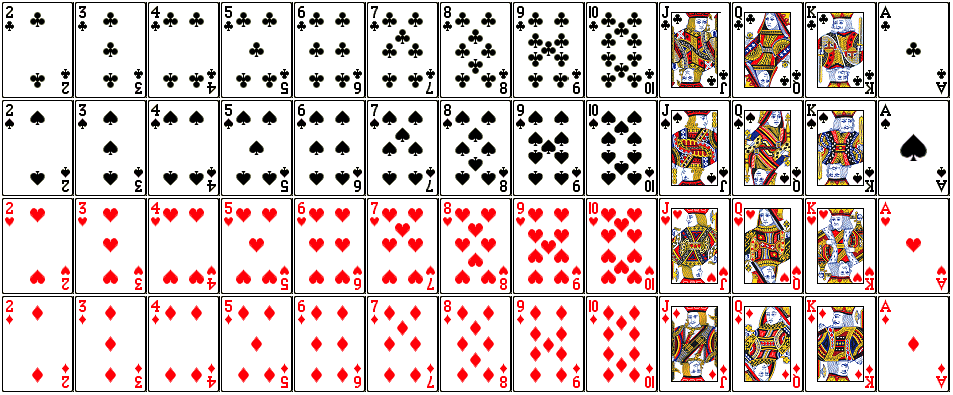
\includegraphics[scale=0.45]{kort}
	\end{figure}  

\prbxl{0.5}{Tenk at vi trekk opp eit kort frå ein blanda kortstokk. 
	Vi ønsker å finne sannsynet for 'å trekke kløverkort \textsl{eller} honnørkort'.
	Vi startar med å telle opp dei gunstige utfalla for kløverkort, og finn at antalet er 13.}
\qquad
\prbxr{0.4}{Eit kort som kløver kong er eit kløverkort, men det er også eit honnørkort, og derfor er det begge deler; \textsl{både} kløverkort \textsl{og} honnørkor.}
	
	\begin{figure}[H]
		\centering
		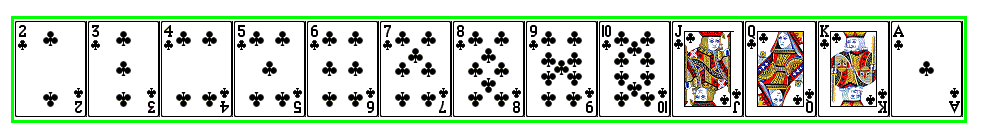
\includegraphics[scale=0.45]{kort1}
	\end{figure}
	Etterpå tell vi opp gunstige utfall for honnørkort, og finn at antalet er 16. \\
	\begin{figure}[H]
		\centering
		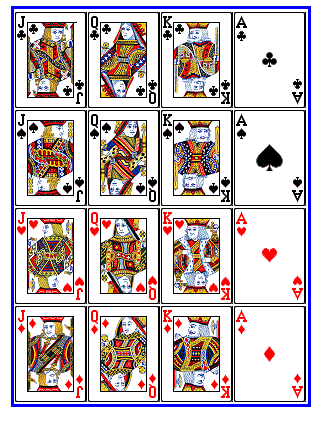
\includegraphics[scale=0.45]{kort2}
	\end{figure}
Til saman har vi telt ${13+16=29}$ gunstige utfall, men no støter vi på eit problem. For da vi fann alle kløverkort, telte vi blant anna kløver knekt, dame, kong og ess. Desse fire korta telte vi også da vi fann alle honnørkort, noko som betyr at vi har telt dei same korta to gongar! \\
	\begin{figure}[H]
		\centering
		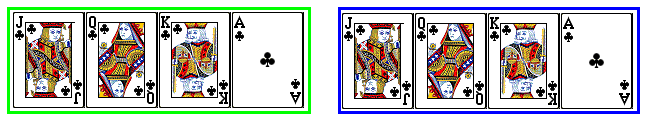
\includegraphics[scale=0.45]{kort4}
	\end{figure}
Det finst no for eksempel ikkje to kløver ess i ein kortstokk, så skal vi rekne ut kvor mange kort som oppfyller kravet om å vere kløver \textsl{eller} honnør, så må vi trekke ifrå antalet kort vi har telt dobbelt:
$$ 13+16-4=25 $$
	\begin{figure}[H]
		\centering
		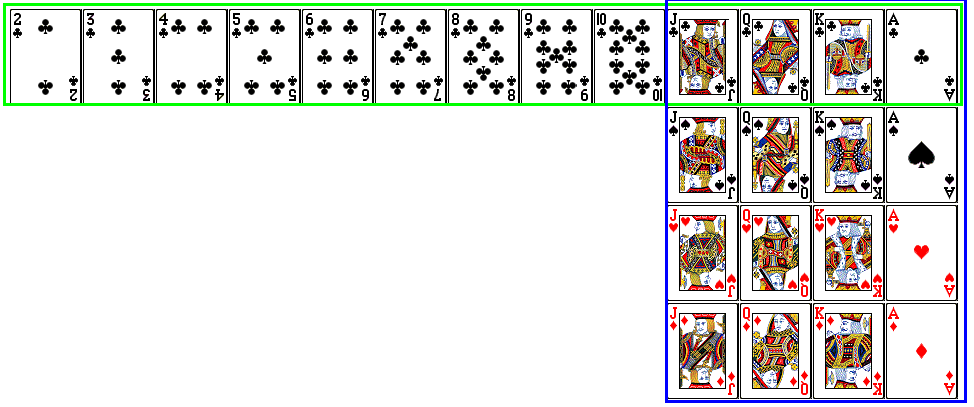
\includegraphics[scale=0.45]{kort3}
	\end{figure}

La \textit{K} vere hendinga 'å trekke eit kløverkort' og \textit{H} være hendinga 'å trekke eit honnørkort'. Sidan det er 25 kort som er kløverkort \textsl{eller} honnørkort av i alt 52 kort, har vi at
$$P(K\cup\,H)=\frac{25}{52}$$

Sidan vi har 13 kløverkort og 16 honnørkort, får vi vidare at
$$P(K)=\frac{13}{52} \text{\; og \;} P(H)=\frac{16}{52}$$
\prbxl{0.6}{
Vi har sett at fire kort er \textsl{både} kløver \textsl{og} honnørkort, dette skriv vi som}\qquad
\prbxr{0.3}{Symbolet \sym{$ \cap $} kallast \textit{snitt}.} \vs
\[ K\,\cap\,H=4 \]
Vi seier da at \textit{K} og \textit{H} har 4 \textit{felles utfall}.
Vidare er
\[ P(K\,\cap\,H)=\frac{4}{52} \]

No som vi har funne $ P(K), P(H)$ og $P(K\cup H)$ kan vi igjen finne  $P(K\,\cap\,H)$ på følgande måte:
\begin{align*}
P(K\,\cup\,H)&=P(K)+P(H)-P(K\,\cap\,H) \br
&= \frac{13}{52}+\frac{16}{52}-\frac{4}{52} \br
&= \frac{25}{52}
\end{align*}

\reg[Hendingar med felles utfall \label{mfutf}]{For to hendingar $ A $ og $ B $ er
	\[ P(A\,\cup\,B)=P(A)+P(B)-P(A\,\cap\,B) \]\vs\vs}
\info{Merk}{
	Viss ein anvender \rref{mfutf} på to hendingar uten felles utfall, ender ein opp med \rref{ufutf}. 
}
\newpage
\eks{ \label{eksfothand}
I ein klasse på 20 personar spelar 7 personar fotball og 10 personar spelar handball. Av desse er det 4 som spelar både fotball og handball. Om ein trekk ut éin person frå klassen, kva er sannsynet for at denne personen spelar fotball \textsl{eller} handball?
		
\sv
Vi lar $ F $ være hendinga 'spelar fotball' og $ H $ vere hendinga 'spelar handball'.
\begin{itemize} 
\item Sannsynet for at ein person spelar fotball er
\[ P(F)=\frac{7}{20} \]
\item Sannsynet for at ein person spelar handball er
\[ P(H)=\frac{10}{20} \]
\item Sannsynet for at ein person spelar \textsl{både} fotball og handball er
\[ P(F\cap H)=\frac{4}{20} \]	
\end{itemize}

Sannsynet for at ein person spelar fotball \textsl{eller} handball er derfor 
\algv{
P(F\cup H)&= P(F)+P(H)-P(F\cap H)\br
&=\frac{7}{20}+\frac{10}{20}-\frac{4}{20}\br
&=\frac{13}{20}
} 
}

\subsection{Venndiagram}
Målet med eit venndiagram er å lage ein figur som illustrerer antalet av dei \textsl{særskilde} utfalla og dei \textsl{felles} utfalla. La oss bruke eksempelet på side \pageref{eksfothand} til å lage ein slik figur. For klassen der nokon spelar fotball, nokon handball og nokon begge deler, kan vi lage eit venndiagram som vist under.
\begin{figure}
	\centering
	\includegraphics[]{\figp{venn}}
\end{figure}
Den grøne ellipsa\footnote{Ei ellipse er ein ''strekt'' sirkel.} representerer dei som spelar fotball ($ F $) og den blå dei som spelar handball ($ H $). Da nokre spelar \textsl{begge} sportane ($ F\cap H $), har vi teikna ellipsane litt over i kvarandre. Videre veit vi at 7 spelar fotball, 10 spelar handball og 4 av disse gjer \textsl{begge} deler. Dette illustrerast slik:
\begin{figure}
	\centering
	\includegraphics[]{\figp{vennb}}
\end{figure}
Diagrammet fortel no at 3 personar spelar \textsl{berre} fotball og 6 spelar \textsl{berre} handball. I tilleg spelar 4 personar \textsl{både} fotball og handball. (Til saman er det derfor 7 som spelar fotball og 10 som spelar handball.) 
\newpage
\eks[1]{I en skuleklasse er det 31 elevar. I denne klassen er det 15 elevar som tek buss til skulen og 9 elever som ter båt. Av desse er det 3 stykker som ter både buss og båt.

\abc{
\item Sett opp eit venndiagram som illustrerer gitt informasjon.\br

\item Éin person trekkast tilfeldig ut av klassen. Kva er sannsynet for at denne personen tar buss \textsl{eller} båt til skulen?
}
\sv
\abc{
\vs	
\item Sidan 3 elevar tek \textsl{både} buss og båt, er det \y{15-3=12} som \textsl{berre} tek buss og \y{9-3=6} som \textsl{berre} tek båt. Vi let $ A $ bety 'tar buss' og $ B $ bety 'tar båt', venndiagrammet vårt blir da sjåande slik ut:
\fig{venne}
\item Sannsynet for at ein person tek buss \textsl{eller} båt kan vi skrive som \y{P(A\cup B) }. Sidan 15 elevar tek buss, 9 ter båt og 3 tek begge deler, er det i alt \y{15+9-3=21} elever som tek buss \textsl{eller} båt. Da det er 31 elevar i alt å velge mellom, er
\[ P(A\cup B)=\frac{21}{31} \]\vs}
}
\newpage
\eks[2]{
Om ein klasse med 29 elevar veit vi følgande:
\begin{itemize}
	\item 16 elevar speler fotball
	\item 12 elevar speler handball
	\item 7 elevar speler volleyball
	\item 5 elevar speler både fotball og handball, men ikkje volleyball
	\item 3 elevar speler både fotball og volleyball, men ikkje handball
	\item 2 elevar speler både handball og volleyball, men ikkje fotball.	
	\item 1 elev speler alle tre sportane.
\end{itemize}
\textbf{a)} Sett opp eit venndiagram som skildrar fordelinga av dei tre sportane i klassen.\br

\textbf{b)} Én person blir tilfeldig trekt ut av klassen. Kva er sannsynet for at denne personen speler enten fotball, handball eller volleyball?\br

\textbf{c)} Personen som blir trekt ut viser seg å spele fotball. Kva er sjansen for at denne personen også speler handball?

\sv
\textbf{a)} La $ F $ bety 'speler fotball', $ H $ bety 'speler handball' og $ V $ bety 'speler volleyball'. Når vi skal lage eit venndiagram, er det lurt å skrive inn dei felles utfalla først. Ut ifrå fjerde til sjuande punkt kan vi teikne dette:
\begin{figure}
	\centering
	\includegraphics[]{\figp{venn3ea}}
\end{figure}
Da ser vi videre at \y{16-5-1-3=7} elevar speler \textsl{berre} fotball, \y{12-5-1-2=4} speler \textsl{berre} handball og \y{9-3-1-2=3} speler \textsl{berre} volleyball:
\begin{figure}
	\centering
	\includegraphics[]{\figp{venn3e}}
\end{figure} 
\textbf{b)} Av diagrammet vårt ser vi at det er $ 8+5+1+3+4+2+3= 26$ unike elevar som speler éin eller fleire av sportene. Sjansen for å trekke ein av desse 26 i ein klasse med 29 elever er $ \frac{17}{29} $. \br

\textbf{c)} Vi les av diagrammet at av dei totalt 16 som speler fotball, er det \y{5+1=6} som også speler handball. Sjansen for at personen som er trekt ut speler handball er derfor $ \frac{6}{16}=\frac{3}{8} $.
}
\subsection{Krysstabell}
Når det er snakk om to hendingar, kan vi også sette opp ein \textit{krysstabell} for å skaffe oss oversikt. Sei at det på ein skule med 300 elevar blir delt ut mjølk og epler til dei elevane som ønsker det i lunsjen. Sei vidare at 220 av elevane får mjølk, mens 250 får eple. Av desse er det 180 som får både mjølk og eple. Viss vi lar $ M $ bety \textit{får mjølk} og $ E $ bety \textit{får eple}, vil krysstabellen vår først sjå slik ut:
\begin{center}
	\renewcommand{\arraystretch}{1.5}
	\begin{tabular}{|c|c|c|c}
		& M &$ \bar{M} $ & sum \\
		\hline$ E $ & & \\
		\hline$ \bar{E} $ & &\\
		\hline sum & &
	\end{tabular}
\end{center}
Så fyller vi inn tabellen ut ifrå infoen vi har:
\begin{itemize}
	\item får \textsl{både} mjølk og eple: \y{M\cap E = 180}
	\item får mjølk, men ikkje eple: \y{M\cap \bar{E} = 220-180=40}
	\item får eple, men ikkje mjølk: \y{E\cap M=250-180=70}
	\item får verken mjølk eller eple: \y{\bar M \cap\bar{E}=300-180-40-70=10}
\end{itemize}

\begin{center}
	\renewcommand{\arraystretch}{1.5}
	\begin{tabular}{|c|c|c|c}
				& M &$ \bar{M} $ & sum \\
		\hline$ E $ & 180& 70&250 \\
		\hline$ \bar{E} $ & 40 &10&50\\
		\hline sum & 220& 80& 300
	\end{tabular}
\end{center}

\section{Gjentatte trekk \label{komb}}
\subsection{Permutasjoner}
\begin{figure}[H]
	\centering
	\includegraphics[scale=0.8]{\figp{bolle}}
	\vs
\end{figure}
Sei vi har en bolle med fire kuler som er nummererte frå 1 til 4. I eit forsøk trekk vi opp ei og ei kule fram til vi har trekt opp tre kuler. Viss vi for eksempel først trekk kule 2, deretter kule 4, og så kule 3, får vi \textit{permutasjonen} $2\; 4\; 3$. \vsk
 
Kor mange forskjellige permutasjoner kan vi få? La oss lage ein figur som hjelper oss med å finne svaret. Ved første trekning er det 4 kuler å plukke av, vi kan derfor seie at vi har 4 vegar å gå. Enten trekk vi kule 1, eller kule 2, eller kule 3, eller kule 4:
\begin{figure}[H]
\centering
\includegraphics[scale=0.8]{\figp{perm1a}}
\end{figure}
Kula vi trekk opp, legg vi ut av bollen, og trekk så for andre gang. For kvar av de 4 vegane vi kunne gå i første trekning får vi no 3 nye vegar å gå. Altså har vi nå  $3\cdot4=12$ vegar vi kan gå.

\begin{figure}[H]
	\centering
	\includegraphics[scale=0.8]{\figp{perm1b}}
\end{figure}
 
Den andre kula vi trekk opp legg vi også ut av bollen,  så for kvar av dei 12 vegane fra 2. trekning, får vi no to nye moglege vegar å gå. Totalt antall vegar (permutasjoner) blir derfor $12\cdot2=24$. 

\begin{figure}[H]
\centering
\includegraphics[scale=0.8]{\figp{perm1c}}
\end{figure}

Denne utrekninga kunne vi også ha skrive slik:
\[ 4\cdot3\cdot2=24 \]
\reg[Produktregelen for permutasjonar]{Når vi gjer fleire trekningar etter kvarandre, finn vi alle moglege permutasjonar ved å gonge saman antall moglege utfall i kvar trekning.
}

\eks{	
	Av dei 29 bokstavene i alfabetet ønsker vi å lage eit ord som består av 3 bokstavar. Vi godkjenner ord som ikkje har noko tyding, men ein bokstav kan berre brukast éin gang i ordet.\os
	
	Kor mange ord kan vi lage?

	\sv
	Først har vi 29 bokstavar å trekke fra, deretter 28 bokstavar, og til slutt 27 bokstavar. Dermed er antall permutasjonar gitt som
	\[ \underbrace{29}_{\substack{\text{moglege utfall}\\\text{1. trekning}}}\cdot\underbrace{28}_{\substack{\text{moglege utfall}\\\text{2. trekning}}}\cdot\underbrace{27}_{\substack{\text{moglege utfall}\\\text{3. trekning}}}=21\,924 \]
	Vi kan altså lage 21\,924 forskjellige ord.
}
\eks[2]{
	Vi kastar om krone eller mynt fire gongar etter kvarandre. Kor mange permutasjoner har vi da?
	
	\sv
	Kvar gong vi kaster om krone eller mynt, har vi to moglege utfall. Antall permutasjoner er derfor gitt som
	\[ 2\cdot2\cdot2\cdot2=16 \]\vs}
\newpage
\info{Kombinasjonar}{
I dagligtale blir ofte ordet \textit{kombinasjonar} brukt i staden for permutasjonar, men innan sannsynsrekning har kombinasjonar og permutasjonar forskjellig tyding. Den store forskjellen er at permutasjonar tar hensyn til rekkefølge, mens kombinasjonar ikkje gjer det. \vsk

Sei vi ønsker å danne eit ord med to bokstaver ved hjelp av med bokstavene $ A $, $ B $ og $ C $, og at vi godtar gjenbruk av bokstav. Da har vi 9 moglege permutasjonar:
\[ AA, AB, AC, BB, BA, BC, CC, CA, CB \]
Kombinasjonar derimot viser til ei unik samansetting når rekkefølge ikkje blir teke hensyn til, for eksempel er $ AB $ og $ BA $ den samme kombinasjonen. I dette tilfellet har vi altså 6 kombinasjonar
\[ AA, AB, AC, BB, BC, CC \]
}
\newpage
\subsection{Sannsyn ved gjentatte trekk}
\prbxl{0.5}{Tenk at vi har ein med bolle sju kuler. Tre av dei er grøne, to er blå og to er raude. Sei at vi tar opp først éi kule av bollen, og deretter éi til. Kva er sannsynet for at vi trekker opp to grøne kuler?} \qquad
\fgbxr{0.4}{
\fig{bolle2}
}
Viss vi lar $ G $ bety 'å trekke ei grøn kule', kan vi skrive dette sannsynet som $ P(GG) $. For å komme fram til eit svar, startar vi med å finne ut kor mange \textsl{gunstige} permutasjoner vi har. Sidan vi i første trekning har 3 gunstige utfall, og i andre trekning 2 gunstige utfall, har vi $3\cdot2=6$ gunstige permutasjonar. Totalt velg vi blant 7 kuler i første trekning og 6 kuler i andre trekning. Antal \textsl{moglege} permutasjonar er derfor $7\cdot6=42$\,. Sannsynet for å få to grøne kuler blir da
\begin{equation}
P(GG)=\frac{3\cdot2}{7\cdot6}=\frac{6}{42}=\frac{1}{7} \label{trekk}
\end{equation}
\rule{\linewidth}{1pt}
La oss også finne sannsynet for å få ei grøn kule for kvar trekning isolert sett. I første trekning har vi 3 grøne av i alt 7 kuler, altså er
\[ P(G)=\frac{3}{7} \]
\prbxl{0.5}{I andre trekning blir det tatt for gitt at ei grønn kule er plukka opp ved første trekning, og dermed er ute av bollen. Vi har da 2 av 6 kuler som er grøne:
\[ P(G|G)=\frac{2}{6} \]
}
\qquad
\prbxr{0.4}{Symbolet \sym{$ | $} betyr \textit{\textsl{gitt} at ... har skjedd}. $ P(G|G) $ er derfor en forkortelse for 'sannsynet for å trekke en grøn kule, \textsl{gitt} at ei grøn kule er trukke'.}


Viss vi gongar sannsynet fra første trekning med sannsynet frå andre trekning, blir reknestykket det same som i likning \eqref{trekk}:
\[ P(GG)=\frac{3}{7}\cdot\frac{2}{6}=\frac{6}{42}=\frac{1}{7} \]

\reg[Sannsyn ved gjentatte trekk \label{permsans}]{Sannsynet for at $ A $ vil skje, \textsl{gitt} at $ B$ har skjedd, skrivast som \y{P(A|B)}. \vsk\\

Sannsynet for at $ A $ skjer først, deretter $ B $, deretter $ C $, og så vidare ($ ... $) er
\[ P(ABC...)=P(A)\cdot P(B|A)\cdot P(C|AB)\cdot... \]
}

\eks{
	I ein bolle ligg to blå og to raude kuler.  Vi trekk éi og éi kule opp av bollen, fram til vi har henta opp tre kuler. Kva er sannsynet for at vi først trekk ei blå, deretter in raud, og til slutt ei blå kule? 
		
		\sv 
		Vi lar  $ B $ bety  'å trekke blå kule' og  $ R $ bety 'å trekke raud kule'. Sannsynet for først ei blå, så ei raud, og så ei blå kule, skriv vi da som $P(BRB)$.
		\begin{itemize}
			\item 	Sannsynet for \textit{B} i første trekning er $P(B)=\frac{2}{4}$.
			\item Sannsynet for \textit{R} i andre trekning, \textsl{gitt} \textit{B} i første er
			\[ P(R|B)=\frac{2}{3} \]
			
			\item Sannsynet for \textit{B} i tredje trekning, \textsl{gitt} \textit{B} i første og \textit{R} i andre er
			\[ P(B|RB)=\frac{1}{2} \]
		\end{itemize}
	  Altså har vi at
		\begin{align*}
		P(BRB)&=P(B)\cdot P(R|B)\cdot P(B|RB)\br
		&= \frac{2}{4}\cdot\frac{2}{3}\cdot\frac{1}{2} \br
		&= \frac{4}{24} \br
		&= \frac{1}{6}
		\end{align*}}

\subsection{Valgtre}
Vi kan utnytte \rref{permsans} for å lage ei hjelpeteikning når vi har å gjere med gjentatte trekk. Teikninga vi her skal ende opp med kallast eit \textit{valgtre}. Vi teikner da ei lignende figur som vi gjor i delkapittel \ref{komb}, men langs alle vegar skriv vi på sannsynet for utfallet vegen leder oss til. 
\begin{figure}[H]
\centering
\includegraphics{\figp{bolle2}}
\end{figure}
La oss igjen sjå på bollen med de sju kulene. Trekk av grøn, blå eller raud kule tegnsett vi høvesvis med bokstavene \textit{G}, \textit{B} og \textit{R}.\vsk

Ved første trekning er sjansen for å trekke en grønn kule $ \frac{3}{7} $, derfor skriver vi denne brøken på veien som fører oss til \textit{G}. Gitt at vi har trekt en grønn kule, er sannsynet for også å trekke en grønn kule i andre trekning lik $ \frac{2}{6} $. Denne brøken skriver vi derfor langs veien som fører oss fra \textit{G} til \textit{G}. Og sånn fortset vi til vi har ført opp alle sannsyna til kvar veg. For å få ei rask oversikt over dei forskjellige permutasjonane vegane fører til, kan det være lurt å skrive opp desse under kvar ende av treet.  \vs
\begin{figure}[H]
\centering
\includegraphics[]{\figp{tree}}
\end{figure}
La oss no bruke valgtreet over til å finne sannsynet for å trekke éi grøn og éni blå kule. \textit{GB} og \textit{BG} er da dei gunstige permutasjonane. Ved å gonge saman sannsyna langs vegen til \textit{GB}, finn vi at
\[ P(GB)=\frac{3}{7}\cdot\frac{2}{6}=\frac{6}{42} \]
På samme måte kan vi finne \textit{P(BG)}:
\[ P(BG)=\frac{2}{7}\cdot\frac{3}{6}=\frac{6}{42} \]
Sannsynet for at '\textit{GB} \textsl{eller} \textit{BG}' inntreff er (sjå \rref{mfutf}):
\begin{align*}
P(GB\cup BG)&=P(GB)+P(BG) \\
		&=\frac{6}{42}+\frac{6}{42} \br
		&= \frac{12}{42} \br
		&= \frac{2}{7}
\end{align*}


\reg[Permutasjonar på eit valgtre]{For å finne sannsynet til ein permutasjon på eit valgtre, gongar vi saman sannsyna langs vegen vi må følge for å kome til permutasjonen. }
\eks{I ein bolle med 10 kuler er tre kuler grøne, to er blå og fem er raude. Du trekk to kuler ut av bollen. La $ G, B $ og $ R $ høvesvis bety 'å trekke ei blå kule', 'å trekke ei grøn kule' og 'å trekke ei raud kule'.\vsk

\textbf{a)}  Teikn eit valgtre som skisserer permutasjonane av $ B $, $ G $ og $ R $ du kan få.	\br
\textbf{b)} Kva er sannsynet for at du trekk to raude kuler? \br
\textbf{c)} Kva er sannsynet for at du trekk éi blå og éi grøn kule? \br
\textbf{d)} Kva er sannsynet for at du trekk \textsl{minst} éi blå \textsl{eller minst} éi  grønn kule?

\sv
\textbf{a)}
\begin{figure}[H]
	\centering
	\includegraphics{\figp{treee}}
\end{figure}
\textbf{b)} Av valgtreet vårt ser vi at
\alg{
	P(RR)&=\frac{2}{10}\cdot\frac{1}{9}\br
	&= \frac{2}{90} \br
	&= \frac{1}{45}
}
\textbf{c)} Både permutasjonen $ GB $ og $ BG $ gir oss éi blå og éi grønn kule. Sannsynet for kvar av dei er
\alg{
P(GB)&= \frac{3}{10}\cdot\frac{5}{9} \br
&= \frac{15}{90} \br
&= \frac{1}{6}
}
\alg{
P(BG) &= \frac{5}{10}\cdot\frac{3}{9} \br
&= \frac{1}{6}
}
Sannsynet for $ GB $ \textsl{eller} $ BG $ er summen av $ P(GB) $ og $ P(BG) $:
\alg{
P(GB\cup BG) &= P(GB)+P(BG) \\
&= \frac{1}{6}+\frac{1}{6} \br
&= \frac{2}{6} \br
&= \frac{1}{3}
}
\textbf{d)} For å svare på denne oppgåva kan vi sjølvsagt legge saman sannsynet for permutasjonane $ GG $, $ GB $, $ GR$, $ BG $, $ BB $, $ BR $, $ RG $ og $ RB $, men vi sparer oss veldig mykje arbeid viss vi merker oss dette: Å få \textsl{minst} én blå \textsl{eller minst} én grønn kule er det motsatte av å \textsl{berre} få raude kuler. Sannsynet for dette, å få to raude kuler, fant vi i oppgave b). Av \rref{motsatt} har vi at
\alg{
P(\bar{R}) &= 1-P(R) \br
&= 1- \frac{1}{45} \br
&= \frac{45}{45}-\frac{1}{45} \br
&= \frac{44}{45}
}
Sannsynet for å få \textsl{minst} én blå \textsl{eller minst} éi grøn kule er altså $ \frac{44}{45} $.
}

\end{document}


